% Options for packages loaded elsewhere
\PassOptionsToPackage{unicode}{hyperref}
\PassOptionsToPackage{hyphens}{url}
\PassOptionsToPackage{dvipsnames,svgnames*,x11names*}{xcolor}
%
\documentclass[
  10pt,
  ignorenonframetext,
  aspectratio=43,
]{beamer}
\usepackage{pgfpages}
\setbeamertemplate{caption}[numbered]
\setbeamertemplate{caption label separator}{: }
\setbeamercolor{caption name}{fg=normal text.fg}
\beamertemplatenavigationsymbolsempty

%%
%%% Definition of colors
%%% Source: https://latexcolor.com/
\definecolor{blanchedalmond}{rgb}{1.0, 0.92, 0.8}
\definecolor{blond}{rgb}{0.98, 0.94, 0.75}
%%% End of definition of colors
%%

% Prevent slide breaks in the middle of a paragraph
\widowpenalties 1 10000
\raggedbottom
\usepackage{lmodern}
\usepackage{amssymb,amsmath}
\usepackage{ifxetex,ifluatex}
\ifnum 0\ifxetex 1\fi\ifluatex 1\fi=0 % if pdftex
  \usepackage[T1]{fontenc}
  \usepackage[utf8]{inputenc}
  \usepackage{textcomp} % provide euro and other symbols
\else % if luatex or xetex
  \usepackage{unicode-math}
  \defaultfontfeatures{Scale=MatchLowercase}
  \defaultfontfeatures[\rmfamily]{Ligatures=TeX,Scale=1}
  \setmainfont[]{Myriad Pro}
  \ifxetex
    \usepackage{xeCJK}
    \setCJKmainfont[ItalicFont=AR PL UKai TW]{AR UDJingXiHeiPU30}
  \fi
  \ifluatex
    \usepackage[]{luatexja-fontspec}
    \setmainjfont[ItalicFont=AR PL UKai TW]{AR UDJingXiHeiPU30}
  \fi
\fi
\usetheme[]{metropolis}
\usecolortheme{default}
\usefonttheme{serif} % use mainfont rather than sansfont for slide text
% Use upquote if available, for straight quotes in verbatim environments
\IfFileExists{upquote.sty}{\usepackage{upquote}}{}
\IfFileExists{microtype.sty}{% use microtype if available
  \usepackage[]{microtype}
  \UseMicrotypeSet[protrusion]{basicmath} % disable protrusion for tt fonts
}{}
\makeatletter
\@ifundefined{KOMAClassName}{% if non-KOMA class
  \IfFileExists{parskip.sty}{%
    \usepackage{parskip}
  }{% else
    \setlength{\parindent}{0pt}
    \setlength{\parskip}{6pt plus 2pt minus 1pt}}
}{% if KOMA class
  \KOMAoptions{parskip=half}}
\makeatother
\usepackage{xcolor}
\IfFileExists{xurl.sty}{\usepackage{xurl}}{} % add URL line breaks if available
\IfFileExists{bookmark.sty}{\usepackage{bookmark}}{\usepackage{hyperref}}
\hypersetup{
  pdftitle={Reserving Female Status --- Women Reserved Seats and Gender Empowerment in Taiwan},
  pdfauthor={Yu-Hsin Ho},
  colorlinks=true,
  linkcolor=Maroon,
  filecolor=Maroon,
  citecolor=Blue,
  urlcolor=red,
  pdfcreator={LaTeX via pandoc}}
\urlstyle{same} % disable monospaced font for URLs
\newif\ifbibliography
\usepackage{listings}
\newcommand{\passthrough}[1]{#1}
\lstset{defaultdialect=sh}
\lstset{framexleftmargin=0mm, frame=trBL,backgroundcolor=\color{blanchedalmond!5},numbers=left,numberstyle=\scriptsize,basicstyle=\small}
\lstset{aboveskip=5mm,belowskip=5mm,xleftmargin=20pt,xrightmargin=5pt}
% \lstset{prebreak={\raisebox{0ex}[0ex][0ex]}}
% \lstset{postbreak={\raisebox{0ex}[0ex][0ex]\space}}
\lstset{breaklines=true,breakatwhitespace=true}
\usepackage{longtable,booktabs}
\usepackage{graphicx,grffile}
\makeatletter
\def\maxwidth{\ifdim\Gin@nat@width>\linewidth\linewidth\else\Gin@nat@width\fi}
\def\maxheight{\ifdim\Gin@nat@height>\textheight\textheight\else\Gin@nat@height\fi}
\makeatother
% Scale images if necessary, so that they will not overflow the page
% margins by default, and it is still possible to overwrite the defaults
% using explicit options in \includegraphics[width, height, ...]{}
\setkeys{Gin}{width=\maxwidth,height=\maxheight,keepaspectratio}
% Set default figure placement to htbp
\makeatletter
\def\fps@figure{htbp}
\makeatother
\setlength{\emergencystretch}{3em} % prevent overfull lines
\providecommand{\tightlist}{%
  \setlength{\itemsep}{0pt}\setlength{\parskip}{0pt}}
\setcounter{secnumdepth}{-\maxdimen} % remove section numbering

%
% When using babel or polyglossia with biblatex, loading csquotes is recommended 
% to ensure that quoted texts are typeset according to the rules of your main language.
%
\usepackage{csquotes}

%
% blockquote
%
\definecolor{blockquote-border}{RGB}{221,221,221}
\definecolor{blockquote-text}{RGB}{89,89,89}
\usepackage{mdframed}
\newmdenv[rightline=false,bottomline=false,topline=false,linewidth=3pt,linecolor=blockquote-border,skipabove=\parskip]{customblockquote}
\renewenvironment{quote}{\begin{customblockquote}\list{}{\rightmargin=0em\leftmargin=0em}%
\item\relax\color{blockquote-text}\ignorespaces}{\unskip\unskip\endlist\end{customblockquote}}

%
% Source Sans Pro as the de­fault font fam­ily
% Source Code Pro for monospace text
%
% 'default' option sets the default 
% font family to Source Sans Pro, not \sfdefault.
%

\usepackage{tikz}
\usepackage{pgfplots}
\usepackage{adjustbox}
\usepackage{booktabs}
\linespread{1.3}
\usepackage{array}

\title{Reserving Female Status --- Women Reserved Seats and Gender
Empowerment in Taiwan}
\author{Yu-Hsin Ho}
\date{May 28, 2022}
\institute{Department of Economics, National Taiwan University}

\begin{document}
\frame{\titlepage}

\hypertarget{background}{%
\section{Background}\label{background}}

\begin{frame}{Background}
General discussion around gender quota policy:

\begin{enumerate}
\tightlist
\item
  \textbf{Empathy/Information Provision}: exposure improves
  understanding, updating prior belief to reduce statistical
  discrimination
\item
  \textbf{Backlash}: ``reverse discrimination'', threatened status for
  privileged group
\end{enumerate}
\end{frame}

\begin{frame}{A Progressive Gender Perspective of \emph{ROC
Consitution}}
\protect\hypertarget{a-progressive-gender-perspective-of-roc-consitution}{}
\begin{quote}
\emph{中華民國憲法第 134 條}

各種選舉,應規定婦女當選名額,其辦法以法律定之。
\end{quote}

\begin{itemize}
\tightlist
\item
  Mandatory women reserved seats in \emph{any} election codified in
  \emph{ROC Constitution} since 1946
\item
  Local council elections in Taiwan reserved 1 woman seat per 4 elected
  member (or per 5 before 1999)

  \begin{itemize}
  \tightlist
  \item
    Guaranteeing 14\% \textasciitilde{} 25\% female representatives for
    electoral districts having \(\geq\) 4 members
  \end{itemize}
\item
  The lowest voted male winner will be replaced by highest voted female
  candidate if the requirement doesn't meet.
\end{itemize}
\end{frame}

\begin{frame}
Past researches on effects of women political representation utilized a
natural experiment in India

\begin{block}{1993 Constitution Amendment in India}
\protect\hypertarget{constitution-amendment-in-india}{}
\begin{itemize}
\tightlist
\item
  1/3 seats reserved for women in local council elections
\item
  Higher female political representation due to this policy
\item
  \textbf{Identification}: States adopting this policy was designated
  randomly, causing random treatment and time variation
\end{itemize}
\end{block}
\end{frame}

\hypertarget{data-and-identification-strategy}{%
\section{Data and Identification
Strategy}\label{data-and-identification-strategy}}

\begin{frame}{Data and Identification Strategy}
\begin{block}{Outcomes: Son Preference}
\protect\hypertarget{outcomes-son-preference}{}
\begin{enumerate}
\tightlist
\item
  Having 3rd child
\item
  Sex ratio of 3rd parity
\end{enumerate}

From MOI Newborns Data between 1998 and 2006

\begin{itemize}
\tightlist
\item
  Samples: Couples who already have 2 children, deciding whether to have
  3rd one.
\item
  Transformed into balanced panel data by couple and year
\end{itemize}
\end{block}
\end{frame}

\begin{frame}
\begin{figure}
\centering
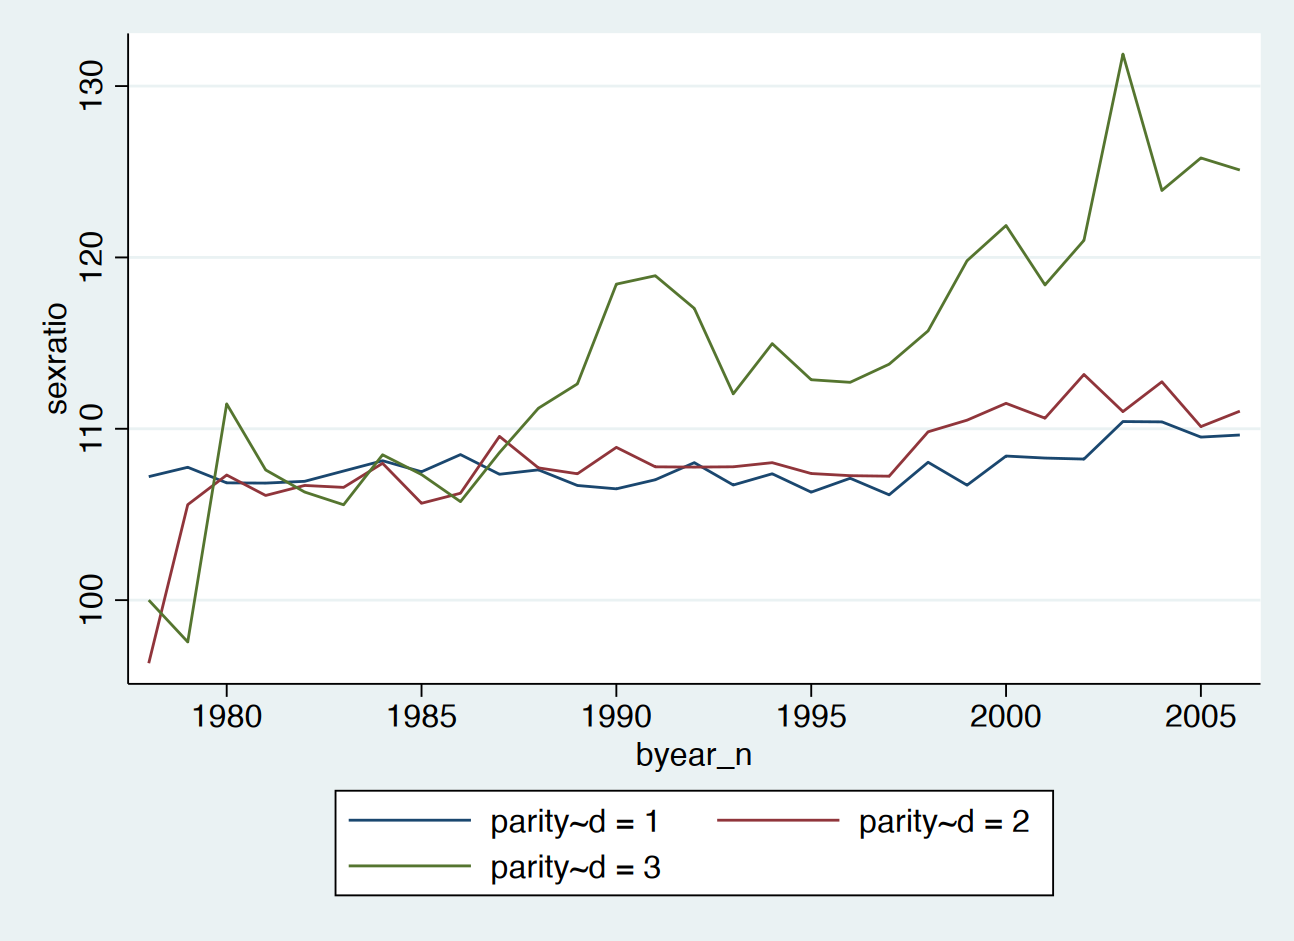
\includegraphics[width=0.8\textwidth,height=\textheight]{graphs/sexratioByParity.png}
\caption{Newborns Sex Ratio by Parity}
\end{figure}
\end{frame}

\begin{frame}
\begin{block}{Survey Outcomes: Son Preference \& Gender Role}
\protect\hypertarget{survey-outcomes-son-preference-gender-role}{}
Taiwan Social Change Survey

\begin{itemize}
\tightlist
\item
  Sample: Period 2001, 2006

  \begin{enumerate}
  \tightlist
  \item
    「為傳宗接代,至少要生一兒子」
  \item
    「一個家庭幾個小孩最理想」
  \end{enumerate}
\item
  Sample: Period 2011, 2016

  \begin{itemize}
  \tightlist
  \item
    Gender role variables
  \end{itemize}
\end{itemize}
\end{block}
\end{frame}

\begin{frame}
Vote data from 1998, 2002, 2005 council elections.

\begin{block}{Instrument: \% of reserved seats}
\protect\hypertarget{instrument-of-reserved-seats}{}
\begin{itemize}
\tightlist
\item
  \(Z_{ed} = \frac{\text{Reserved Seats 保留名額數}}{\text{Member Size 應選人數}}\),
  in election year \(e\), electoral district \(d\)
\item
  Determined by population size of electoral district.
\end{itemize}
\end{block}

\begin{block}{Potential Treatments}
\protect\hypertarget{potential-treatments}{}
\begin{itemize}
\tightlist
\item
  \% female elected
\item
  \% female candidates
\end{itemize}

Both could affect outcomes. Exclusion restriction not satistied. Thus
I'll present 1st stage and reduced form.
\end{block}
\end{frame}

\begin{frame}{1st Stage Estimations}
\protect\hypertarget{st-stage-estimations}{}
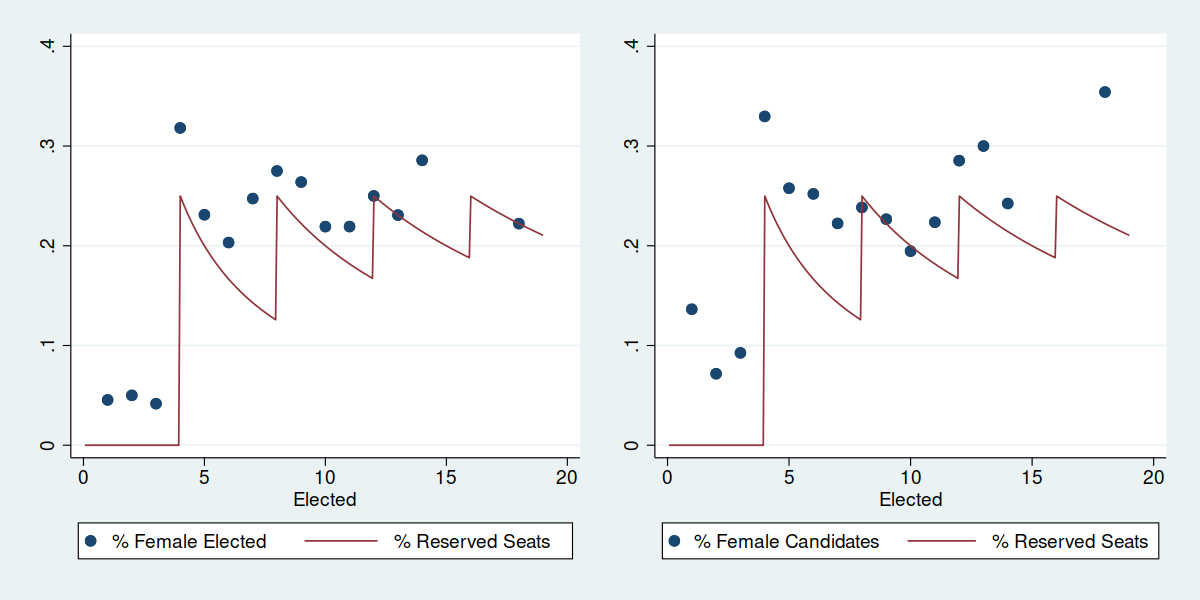
\includegraphics{graphs/firstStage.png}\\

Control for population size to prevent OVB.
\end{frame}

\begin{frame}
\begin{block}{1st Stage Estimations}
\protect\hypertarget{st-stage-estimations-1}{}
\[
X_{td} = \alpha + \beta_1 \text{\% Reserved Seats}_{td}  + \gamma_1 \ln \operatorname{pop}_{tc} + \delta_t + \delta_{c}
\]

in election year \(t\), district \(d\), county \(c\)
\end{block}
\end{frame}

\begin{frame}
\begin{table}
    \caption{1st Stage}
    {
        \def\sym#1{\ifmmode^{#1}\else\(^{#1}\)\fi}
        \begin{tabular}{l*{2}{c}}
            \toprule
                               & \multicolumn{1}{c}{(1)}               & \multicolumn{1}{c}{(2)}                  \\
                               & \multicolumn{1}{c}{\% Elected Female} & \multicolumn{1}{c}{\% Female Candidates} \\
            \midrule
            \% Reserved Seats  & 1.029\sym{***}                        & 0.758\sym{***}                           \\
                               & (0.0620)                              & (0.0578)                                 \\
            Population Control & Yes                                   & Yes                                      \\
            Election Year FE   & Yes                                   & Yes                                      \\
            County FE          & Yes                                   & Yes                                      \\
            \midrule
            Observations       & 2210                                  & 2210                                     \\
            \bottomrule
            \multicolumn{3}{l}{\footnotesize Standard errors in parentheses}                                      \\
            \multicolumn{3}{l}{\footnotesize \sym{*} \(p<0.05\), \sym{**} \(p<0.01\), \sym{***} \(p<0.001\)}      \\
        \end{tabular}
    }
\end{table}
\end{frame}

\hypertarget{results}{%
\section{Results}\label{results}}

\begin{frame}{Results}
Reduced form specification: \[
Y_{itcd} = \alpha + \rho_1 \text{\% Reserved Seats}_{td}  + \gamma_1 \ln \operatorname{pop}_{tc} + X_i' \eta + \delta_t + \delta_{c}
\]

for couple \(i\), year \(t\), county \(c\), electoral district \(d\)
\end{frame}

\begin{frame}{Birth Outcome: Having 3rd Child}
\protect\hypertarget{birth-outcome-having-3rd-child}{}
\begin{table}
    \caption{Outcome: 3rd Child Now}
    {
        \def\sym#1{\ifmmode^{#1}\else\(^{#1}\)\fi}
        \scalebox{0.7}{
            \begin{tabular}{l*{5}{c}}
                \toprule
                                                        & \multicolumn{1}{c}{(1)}         & \multicolumn{1}{c}{(2)}         & \multicolumn{1}{c}{(3)}    & \multicolumn{1}{c}{(4)}   & \multicolumn{1}{c}{(5)}       \\
                                                        & \multicolumn{1}{c}{Full Sample} & \multicolumn{1}{c}{High School} & \multicolumn{1}{c}{Non-HS} & \multicolumn{1}{c}{Urban} & \multicolumn{1}{c}{Non-Urban} \\
                \midrule
                \% Reserved Seats                       & \num{-0.00864}\sym{***}               & \num{-0.00568}                        & \num{-0.0157}\sym{***}           & \num{-0.00898}                  & \num{-0.00690}\sym{**}              \\
                                                        & (\num{0.00289})                       & (\num{0.00417})                       & (\num{0.00301})                  & (\num{0.00719})                 & (\num{0.00309})                     \\
                Daughter Son $\times$ \% Reserved Seats & \num{0.00645}\sym{**}                 & \num{0.00182}                         & \num{0.0160}\sym{***}            & \num{0.0129}\sym{*}             & \num{0.00420}                       \\
                                                        & (\num{0.00263})                       & (\num{0.00403})                       & (\num{0.00284})                  & (\num{0.00713})                 & (\num{0.00285})                     \\
                Son Daughter $\times$ \% Reserved Seats & \num{0.00651}\sym{**}                 & \num{0.00671}                         & \num{0.0125}\sym{***}            & \num{0.0178}\sym{**}            & \num{0.00375}                       \\
                                                        & (\num{0.00261})                       & (\num{0.00417})                       & (\num{0.00268})                  & (\num{0.00681})                 & (\num{0.00280})                     \\
                Both Son $\times$ \% Reserved Seats     & \num{0.00655}\sym{**}                 & \num{0.00570}                         & \num{0.0135}\sym{***}            & \num{0.0178}\sym{***}           & \num{0.00357}                       \\
                                                        & (\num{0.00281})                       & (\num{0.00424})                       & (\num{0.00299})                  & (\num{0.00649})                 & (\num{0.00304})                     \\
                Age, Edu Control                        & Yes                             & Yes                             & Yes                        & Yes                       & Yes                           \\
                Log-Population Control                  & Yes                             & Yes                             & Yes                        & Yes                       & Yes                           \\
                Year FE                                 & Yes                             & Yes                             & Yes                        & Yes                       & Yes                           \\
                County FE                               & Yes                             & Yes                             & Yes                        & Yes                       & Yes                           \\
                \midrule
                Mean                                    & \num{0.00969}                         & \num{0.0126}                          & \num{0.00715}                    & \num{0.00699}                   & \num{0.0105}                        \\
                Observations                            & \num{6654418}                         & \num{3088955}                         & \num{3565463}                    & \num{1525767}                   & \num{5128651}                       \\
                Adj. R-square                           & \num{0.0145}                          & \num{0.0153}                          & \num{0.0130}                     & \num{0.00928}                   & \num{0.0155}                        \\
                \bottomrule
                \multicolumn{6}{l}{\footnotesize Standard errors in parentheses, clustered on year-township}                                                                                                                                     \\
                \multicolumn{6}{l}{\footnotesize \sym{*} \(p<0.1\), \sym{**} \(p<0.05\), \sym{***} \(p<0.01\)}                                                                                                       \\
            \end{tabular}
        }
    }
\end{table}
\end{frame}

\begin{frame}{Birth Outcome: 3rd Parity Sex Ratio}
\protect\hypertarget{birth-outcome-3rd-parity-sex-ratio}{}
\begin{table}
    \caption{Outcome: 3rd Parity Sex Ratio}
    {
        \def\sym#1{\ifmmode^{#1}\else\(^{#1}\)\fi}
        \scalebox{0.7}{
            \begin{tabular}{l*{5}{c}}
                \toprule
                                                        & \multicolumn{1}{c}{(1)}         & \multicolumn{1}{c}{(2)}         & \multicolumn{1}{c}{(3)}    & \multicolumn{1}{c}{(4)}   & \multicolumn{1}{c}{(5)}       \\
                                                        & \multicolumn{1}{c}{Full Sample} & \multicolumn{1}{c}{High School} & \multicolumn{1}{c}{Non-HS} & \multicolumn{1}{c}{Urban} & \multicolumn{1}{c}{Non-Urban} \\
                \midrule
                \% Reserved Seats                       & \num{0.0357}                          & \num{0.00469}                         & \num{0.0305}                     & \num{0.261}                     & \num{0.0207}                        \\
                                                        & (\num{0.0463})                        & (\num{0.0631})                        & (\num{0.0719})                   & (\num{0.196})                   & (\num{0.0478})                      \\
                Daughter Son $\times$ \% Reserved Seats & \num{-0.0549}                         & \num{-0.0667}                         & \num{0.0253}                     & \num{-0.213}                    & \num{-0.0446}                       \\
                                                        & (\num{0.0735})                        & (\num{0.0977})                        & (\num{0.112})                    & (\num{0.315})                   & (\num{0.0755})                      \\
                Son Daughter $\times$ \% Reserved Seats & \num{0.0300}                          & \num{0.143}                           & \num{-0.0308}                    & \num{0.104}                     & \num{0.0363}                        \\
                                                        & (\num{0.0690})                        & (\num{0.0969})                        & (\num{0.108})                    & (\num{0.241})                   & (\num{0.0723})                      \\
                Both Son $\times$ \% Reserved Seats     & \num{0.00702}                         & \num{-0.0831}                         & \num{0.175}                      & \num{-0.276}                    & \num{0.0197}                        \\
                                                        & (\num{0.0694})                        & (\num{0.0918})                        & (\num{0.108})                    & (\num{0.258})                   & (\num{0.0716})                      \\
                Age, Edu Control                        & Yes                             & Yes                             & Yes                        & Yes                       & Yes                           \\
                Log-Population Control                  & Yes                             & Yes                             & Yes                        & Yes                       & Yes                           \\
                Year FE                                 & Yes                             & Yes                             & Yes                        & Yes                       & Yes                           \\
                County FE                               & Yes                             & Yes                             & Yes                        & Yes                       & Yes                           \\
                \midrule
                Mean                                    & \num{0.551}                           & \num{0.560}                           & \num{0.537}                      & \num{0.556}                     & \num{0.550}                         \\
                Observations                            & \num{64470}                           & \num{38971}                           & \num{25499}                      & \num{10659}                     & \num{53811}                         \\
                Adj. R-square                           & \num{0.0106}                          & \num{0.0127}                          & \num{0.00638}                    & \num{0.00906}                   & \num{0.0109}                        \\
                \bottomrule
                \multicolumn{6}{l}{\footnotesize Standard errors in parentheses, clustered on year-township}                                                                                                                                     \\
                \multicolumn{6}{l}{\footnotesize \sym{*} \(p<0.1\), \sym{**} \(p<0.05\), \sym{***} \(p<0.01\)}                                                                                                       \\
            \end{tabular}
        }
    }
\end{table}
\end{frame}

\begin{frame}{Survey Outcome: Son Preference}
\protect\hypertarget{survey-outcome-son-preference}{}
From TSCS 2001, 2006.

\begin{table}
    {
        \def\sym#1{\ifmmode^{#1}\else\(^{#1}\)\fi}
        \scalebox{0.8}{
            \begin{tabular}{l*{2}{c}}
                \toprule
                                             & \multicolumn{1}{c}{(1)}    & \multicolumn{1}{c}{(2)}            \\
                                             & \multicolumn{1}{c}{至少生一兒子} & \multicolumn{1}{c}{理想小孩數}          \\
                \midrule
                Reserved Seats \%            & \num{-0.159}                     & \num{-0.623}                             \\
                                             & (\num{0.262})                    & (\num{0.642})                            \\
                女 $\times$ Reserved Seats \% & \num{-0.493}\sym{**}             & \num{0.524}                              \\
                                             & (\num{0.200})                    & (\num{0.765})                            \\
                Age, Edu Control             & Yes                        & Yes                                \\
                Log-Population Control       & Yes                        & Yes                                \\
                Year FE                      & Yes                        & Yes                                \\
                County FE                    & Yes                        & Yes                                \\
                \midrule
                Mean                         & \num{0.460}                      & \num{2.395}                              \\
                Observations                 & \num{3697}                       & \num{1980}                               \\
                Adj. R-square                & \num{0.130}                      & \num{0.0780}                             \\
                \bottomrule
                \multicolumn{3}{l}{\footnotesize Standard errors in parentheses, clustered on year-township}   \\
                \multicolumn{3}{l}{\footnotesize \sym{*} \(p<0.1\), \sym{**} \(p<0.05\), \sym{***} \(p<0.01\)} \\
            \end{tabular}
        }
    }
\end{table}
\end{frame}

\begin{frame}{Survey Outcome: Gender Role}
\protect\hypertarget{survey-outcome-gender-role}{}
From TSCS 2011, 2016; 1 = Pro-female

{
\def\sym#1{\ifmmode^{#1}\else\(^{#1}\)\fi}
\scalebox{0.7}{
    \begin{tabular}{lm{2.5cm}m{2.5cm}m{2.5cm}m{2.5cm}}
        \toprule
                                     & (1)                   & (2)                    & (3)                        & (4)                    \\
                                     & 丈夫的責任就是賺錢,妻子的責任就是照顧家庭 & 如果母親外出工作,對還沒上小學的小孩比較不好 & 當妻子有份全天(職)的工作時,家庭生活總是會受到妨害 & 在經濟不景氣時,女性員工應比男性員工先被解僱 \\
        \midrule
        Reserved Seats \%            & \num{0.140}                 & \num{-0.0324}                & \num{0.106}                      & \num{-0.180}\sym{*}          \\
                                     & (\num{0.130})               & (\num{0.139})                & (\num{0.154})                    & (\num{0.101})                \\
        女 $\times$ Reserved Seats \% & \num{0.231}                 & \num{0.0812}                 & \num{0.219}                      & \num{0.186}                  \\
                                     & (\num{0.214})               & (\num{0.200})                & (\num{0.201})                    & (\num{0.120})                \\
        Age, Edu Control             & Yes                   & Yes                    & Yes                        & Yes                    \\
        Log-Population Control       & Yes                   & Yes                    & Yes                        & Yes                    \\
        Year FE                      & Yes                   & Yes                    & Yes                        & Yes                    \\
        County FE                    & Yes                   & Yes                    & Yes                        & Yes                    \\
        \midrule
        Mean                         & \num{0.565}                 & \num{0.448}                  & \num{0.532}                      & \num{0.866}                  \\
        Observations                 & \num{4057}                  & \num{4024}                   & \num{4031}                       & \num{3970}                   \\
        Adj. R-square                & \num{0.226}                 & \num{0.0187}                 & \num{0.00833}                    & \num{0.0472}                 \\
        \bottomrule
        \multicolumn{5}{l}{\footnotesize Standard errors in parentheses, clustered on year-township}                                        \\
        \multicolumn{5}{l}{\footnotesize \sym{*} \(p<0.1\), \sym{**} \(p<0.05\), \sym{***} \(p<0.01\)}                                      \\
    \end{tabular}
}
}

\end{frame}

\hypertarget{remarks}{%
\section{Remarks}\label{remarks}}

\begin{frame}{Remarks}
\begin{itemize}
\tightlist
\item
  Weaken son preference: Higher satisfaction of current status for
  couples without son.
\item
  Women with lower educational attainment was more susceptible to
  exposure
\item
  Survey confirmed decreasing son preference.
\item
  No significant effect on gender role attitudes.
\end{itemize}
\end{frame}

\begin{frame}{Possible Mechanisms}
\protect\hypertarget{possible-mechanisms}{}
\begin{enumerate}
\item
  Role model effects:

  Interaction between female council member and female voters.
\item
  Policy effects:

  Public good provision, pro-female \& childcare policies.
\end{enumerate}
\end{frame}

\end{document}
